	\subsection{Метод конечных объёмов}
		Суть метода заключается в разбиении расчётной области на множество непересекающихся конечных объёмов (ячеек), для каждого из которых записывается интегральная формулировка законов сохранения.
		\begin{figure}
			\centering
			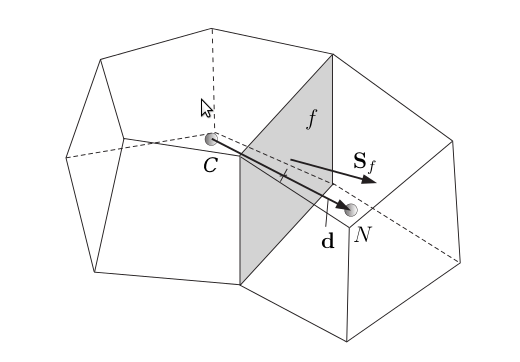
\includegraphics[scale=0.5]{twoCells}
			\caption{Схематическое изображение двух соседних ячеек}
			\label{fig:twoCells}
		\end{figure}
		\subsubsection*{Дискретизация уравнений}
		\addcontentsline{toc}{subsubsection}{Дискретизация уравнений}
		\begin{figure}[ht]
			\begin{minipage}{0.43\linewidth}
				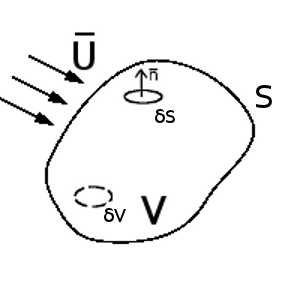
\includegraphics[scale=0.5]{controlVolume}
				\vspace{-2em}
				\caption{Контрольный объём}
				\label{fig:volume}
			\end{minipage}
			\hspace{-1em}
			\begin{minipage}{0.6\linewidth}
				\vspace{-2em}
				Пусть через контрольный объём $V$ \textit{(рисунок \ref{fig:volume})}, ограниченный контрольной поверхностью $S$, $\vec{\delta S} = \vec{n} \delta S$, проходит жидкость со скоростью $\vec{U}$. Выделим бесконечно малый объём $\delta V$. 
			\end{minipage}
		\end{figure}
		Рассмотрим скалярную величину $\Phi$ - плотность распределения некоторой физической величины на единицу массы. Тогда, с учётом того, что $\rho \delta V = \delta m$, в объёме $\delta V$ содержится $\rho \delta V \Phi$ этой физической величины. Уравнение сохранения для этой величины запишется, как
		\begin{equation}
			\frac{\partial}{\partial t} \int_V \rho \Phi \delta V + \oint_S \left( \rho \vec{U} \Phi + \vec{q}_{\Phi}  \right)\cdot \vec{\delta S} = \int_V \rho S_{\phi} \delta V,
			\label{transportEquation}
		\end{equation}
		где $S_{\Phi}$ - суммарная плотность источников, а $\vec{q}_{\Phi}$ -- дифузионный поток. Это уравнение применяется к каждому контрольному объёму. Задача заключается в сведении уравнения (\ref{transportEquation}) к процедуре алгебраического характера.
		
		Введём точку $C$ -- центр ячейки \textit(рисунок \ref{fig:twoCells}) и применим теорему о среднем к объёмному интегралу:
		\begin{figure}[h]
			\begin{minipage}{0.43\linewidth}
				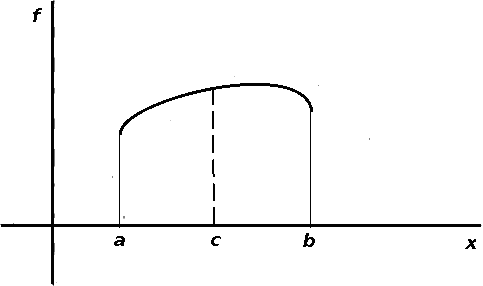
\includegraphics[scale=0.5]{meanValueTheorem}
				\label{fig:meanValueTheorem}
			\end{minipage}
			\hspace{-1em}
			\begin{minipage}{0.6\linewidth}
				\begin{equation}
					\int_a^b fdx \approx f(x_c) \cdot (b-a)
				\end{equation}
				\begin{equation}
					V \frac{\partial \left(\rho \Phi\right)_c}{\partial t} + \oint_S \left( \rho \vec{U} \Phi + \vec{q}_{\Phi}  \right)\cdot \vec{\delta S} = V \left( \rho S_{\Phi} \right)_c
				\end{equation}
				\vspace{2em}
			\end{minipage}
		\end{figure}
			\vspace{-1em}
					
			Пусть контрольная поверхность состоит из граней, то есть имеется огранённый объект. Тогда
			\begin{equation}
				\oint\left(\rho \vec{U} \Phi + \vec{q}_{\Phi} \right) \cdot \vec{\delta S} = \sum_f \int_{S_f} \left(\rho \vec{U} \Phi + \vec{q}_{\Phi} \right) \cdot \vec{\delta S},
			\end{equation}
			где $f$ -- номер грани.
			\begin{equation}
				\int_{S_f} \left(\rho \vec{U} \Phi + \vec{q}_{\Phi} \right) \cdot \vec{\delta S} \approx \left(\rho \vec{U} \Phi + \vec{q}_{\Phi} \right)_f \cdot \vec{S}_f,
			\end{equation}
			где индекс $f$ в выражении $\left(\rho \vec{U} \Phi  + \vec{q}_{\Phi}\right)_f$ означает, что это значение вычисляется в центре грани, а $\vec{S}_f = \vec{n} S_f$. В итоге мы получаем алгебраическое выражение
			\begin{equation}
				V\frac{\partial \left( \rho \Phi \right)_c}{\partial t} + \sum_f \left( \rho \vec{U} \Phi + \vec{q}_{\Phi} \right)_f \cdot \vec{S}_f = V \left( \rho S_{\Phi} \right)_c
			\end{equation}
		\subparagraph{Расчёт диффузионных потоков}
		\begin{equation}
			\int_V \nabla \cdot \left( \Gamma \nabla \Phi \right) \delta V = \int_S \vec{\delta S} \cdot (\Gamma \nabla \Phi) = \sum_f \Gamma_f \vec{S}_f \cdot (\nabla \Phi)_f
		\end{equation}
		\subparagraph{Расчёт ковективных потоков}
		\begin{equation}
			\int_V \nabla \cdot (\rho \vec{U} \Phi) \delta V = \int_S \vec{\delta S} \cdot (\rho \vec{U} \Phi) = \sum_f \vec{S}_f \cdot (\rho \vec{U})_f \Phi_f = \sum_f F \Phi_f
		\end{equation}
		Значение $\Phi_f$ на грани ячейки может быть определено с использованием различных схем:
		
		\textit{Центральная схема (CD)}
		\begin{equation}
		\Phi_f = \beta \Phi_N + (1-\beta)\Phi_C,
		\end{equation}
		где $\beta=\frac{\vec{|CM|}}{\vec{|CM|} + \vec{|NM|}}$ - коэффициент интерполяции, а точка $M$ -- центр грани $f$.
		
		Для коррекции на скошенность ячеек, когда центр грани $f$ не совпадает с пересечением грани $f$ и вектора $\vec{|CP|}$ (точка $M^{'}$), разложим $\Phi_f$ в ряд Тейлора в окрестности точки $M$ и удержим только первые два слагаемых:
		\begin{equation}
			\Phi_M = \Phi_{M^{'}} + \nabla \Phi_{M^{'}} \cdot \vec{M^{'}M} + O\left(\left(M-M^{'}\right)^2\right)
		\end{equation}
		
		\textit{Противопоточная схема (UD)}
		\begin{equation}
			\begin{aligned}
				\Phi_f = \Bigg\{	\begin{array}{l}
					\Phi_P, \quad \text{если } F \geq 0 \\
					\Phi_N, \quad \text{если } F < 0
				\end{array}
			\end{aligned}
		\end{equation}
		
		\textit{Смешанные схемы}
		\begin{equation}
			\Phi_f = \left(1-\gamma\right)(\Phi_f)_{UD} + \gamma (\Phi_f)_{CD},
		\end{equation}
		где коэффициент $\gamma$ меняется в зависимости от конкретной схемы.
		
		\subparagraph{Расчёт градиентов\\}
		
		    Значение градиента может быть вычислено двумя различными способами.
			
			\textit{Метод Гаусса}
			\begin{equation}
				\int_V \nabla \Phi \delta V = \int_S \vec{\delta S} \Phi = \sum_f \vec{S}_f \Phi_f
			\end{equation}
			
			\textit{Метод наименьших квадратов}
			
			Значение $\Phi$ в точке $C$ может быть экстраполировано в соседнюю ячейку с центром в точке $N$ с использованием градиента в точке $C$. Экстраполированное значение в точке $N$ сравнивается с актуальным значением в этой точке и рассчитывается ошибка в определении $\Phi$. Если мы теперь минимизируем сумму квадратов взвешенных ошибок во всех соседних ячейках по отношению к градиенту, значение градиента будет аппроксимировано достаточно точно. Таким образом, вычислив сначала значение тензора
			\begin{equation}
				\mathbf{G} = \sum_N \omega_N^2 (\vec{CN}\vec{CN}),
			\end{equation}
			где весовая функция $\omega = 1/\vec{|CN|}$, а индекс $N$ означает суммирование по всем соседним граням, мы сможем вычислить значение градиента в точке $C$:
			\begin{equation}
				(\nabla \Phi)_C = \sum_N \omega_N^2 \mathbf{G}^{-1} \cdot  (\Phi_N - \Phi_C).
			\end{equation}
	%Метод конечных объёмов
